\subsubsection{power allocation}
% fig
\begin{figure}[t]
\begin{center}
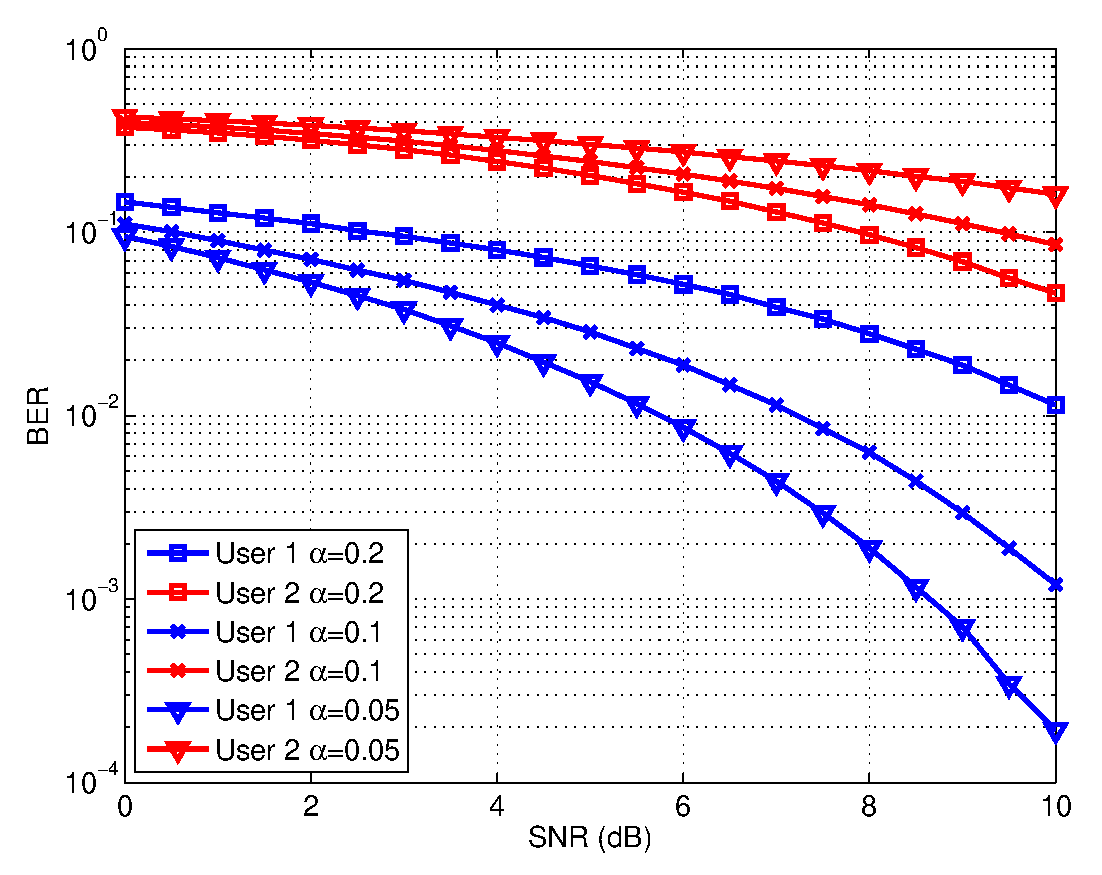
\includegraphics[width=0.95\columnwidth ,angle=0]{figure/snrVSber.eps}
\caption{BER performance of two users with identical channel condition}
\label{fig_sim_snrVSber}
\end{center}
\end{figure}
As in the previous mathematical model, whether or not the desired transmission
signal can be demodulated is not taken into account.
When the base station allocates similar power resources on both users' signals,
the receiver may not be able to extract any of the original data.
In other words, the region where alpha is set near 0.5 have to be checked.
Also, we would like to see the performance of SIC when user 1 and user 2 have
identical channel condition when served by the same base station.

In Fig.~\ref{fig_sim_snrVSber} shows BER curve for 2 users served in same BS 
with same channel condition.
The data stream is multiplexed by power allocation factor $\alpha$ with $0.2$
$0.1$ and $0.05$.
The SNR value is defined as $frac{P}{N_0}$ at receiver end, value $P$ is the
constraint of transmission power of BS as mentioned above.

% fig
\begin{figure}[t]
\begin{center}
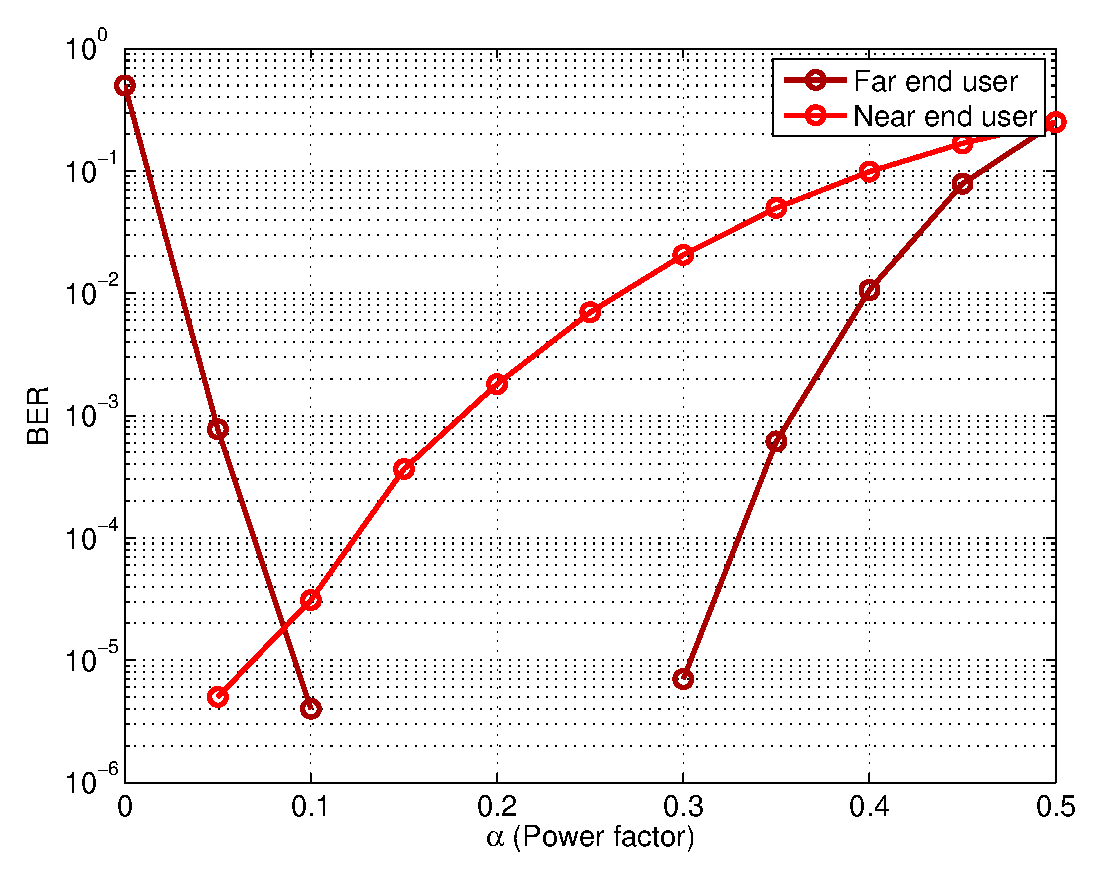
\includegraphics[width=0.95\columnwidth ,angle=0]{figure/alphaVSber.eps}
\caption{BER for different power allocation factor}
\label{fig_sim_aVSber}
\end{center}
\end{figure}
To investigate in the optimal strategy of power allocation, i.e. optimal $\alpha$
value, when serving two users.
In Fig.~\ref{fig_sim_aVSber} shows the BER to different $\alpha$ settings.
The BS transmission power is set to be $5mW/MHz$, and background noise is $-144dBm$.
Near-end user, indexed as user 1, is position at a distance of $150m$, and far-end
user, user 2, is at $220m$.
The channel loss exponent is $4.5$ and thus the PL ratio is about $5.6$.
Supposed that the system requires BER no greater than $10^-2$, $\alpha$
can be set in the range between $0.06$ and $1.17$ in this case.